% !TEX encoding = UTF-8
%Koma article
\documentclass[fontsize=12pt,paper=letter,twoside]{scrartcl}
\usepackage{float}
\usepackage{listings}
\usepackage{makecell}

%Standard Pre-amble
\usepackage[top=4cm,bottom=4cm,left=3cm,right=3cm,asymmetric]{geometry}
%\geometry{landscape}                % Activate for for rotated page geometry
%\usepackage[parfill]{parskip}    % Begin paragraphs with an empty line rather than an indent
\usepackage[table,xcdraw]{xcolor}
\usepackage{graphicx}

\usepackage{amsmath}
\usepackage{amssymb}
\usepackage{epstopdf}
\DeclareGraphicsRule{.tif}{png}{.png}{`convert #1 `dirname #1`/`basename #1 .tif`.png}
% Listings needs package courier
\usepackage{listings} % Needs 
\usepackage{courier}

\usepackage[framemethod=TikZ]{mdframed}
\usepackage{url}

\usepackage{sty/bsymb} %% Event-B symbols
\usepackage{sty/eventB} %% REQ and ENV
\usepackage{sty/calculation}

%Maths
\usepackage{amssymb,amsmath}
\def\Fl{\mathbb{F}}
\def\Rl{\mathbb{R}}
\def\Nl{\mathbb{N}}
\def\Bl{\mathbb{B}}
\def\St{\mathbb{S}}
\newcommand{\ovr}{\upharpoonright}
\newcommand{\var}[1]{\textit{#1}}
%Useful definitions
\newcommand{\mv}[1]{\textit{m\_#1}}
\newcommand{\cv}[1]{\textit{c\_#1}}
\newcommand{\degree}[1]{^{\circ}\mathrm{#1}}
%\newcommand{\comment}[1]{{\footnotesize \quad\texttt{--}\textrm{#1}}}
\newcommand{\im}[1]{i\texttt{-\!#1}}

\usepackage[headsepline]{scrpage2}
\pagestyle{scrheadings}
\ihead[]{\small EECS4312 Report1}
\ohead[]{\small \thepage}
\cfoot[]{}
\ofoot[]{}


%%%%PVS environment%%%%%%%%%%%%%%%%%%%
\lstnewenvironment{pvs}[1][]
    {\lstset{#1,captionpos=b,language=pvs,
    mathescape=true,
    basicstyle=\small\ttfamily,
    numbers=none,
    frame=single,
    % numberstyle=\tiny\color{gray},
    % backgroundcolor=\color{lightgray},
    firstnumber=auto
    }}
    {}
 %%%%%%%%%%%%%%%%%%%%%%%%%%%%%%%%
 
%%%%Verbatim environment%%%%%%%%%%%%%%%%%%%
\lstnewenvironment{code}[1][]
    {\lstset{#1,captionpos=b,
    mathescape=true,
    basicstyle=\small\ttfamily,
    numbers=none,
    frame=single,
    % numberstyle=\tiny\color{gray},
    % backgroundcolor=\color{lightgray},
    firstnumber=auto
    }}
    {}

% \newenvironment{boxed}[1]
%    {\begin{center}
%    #1\\[1ex]
%    \begin{tabular}{|p{0.9\textwidth}|}
%    \hline\\
%    }
%    { 
%    \\\\\hline
%    \end{tabular} 
%    \end{center}
%    }
 %%%%%%%%%%%%%%%%%%%%%%%%%%%%%%%%
 
 %Text in a box
\newenvironment{textbox}
    {\begin{center}
    \begin{tabular}{|p{0.9\textwidth}|}
    \hline\\
    }
    { 
    \\\\\hline
    \end{tabular} 
    \end{center}
    }

\usepackage{hyperref}

%Highlight \hl{}
\usepackage{soul}

\usepackage{enumitem}
\newlist{mylist}{itemize}{1}
\setlist[mylist]{label=\textbullet,leftmargin=1cm,nosep}

\usepackage{multirow}

% Reduce space between figure and caption
%\usepackage{caption}
%\captionsetup[table]{font=small,skip=0pt}     %% Adjust here
%or equivalently 
\usepackage[font=small,skip=4pt]{caption}
%Useful definitions
%\newcommand{\mv}[1]{\textit{m\_#1}}
%\newcommand{\cv}[1]{\textit{c\_#1}}
%\newcommand{\degree}[1]{^{\circ}\mathrm{#1}}
%\newcommand{\comment}[1]{{\footnotesize \quad\texttt{--}\textrm{#1}}}


%For Code Stylings
\usepackage{listings}
\usepackage{color}

\definecolor{dkgreen}{rgb}{0,0.6,0}
\definecolor{gray}{rgb}{0.5,0.5,0.5}
\definecolor{mauve}{rgb}{0.58,0,0.82}

\lstset{frame=tb,
  language=Java,
  aboveskip=3mm,
  belowskip=3mm,
  showstringspaces=false,
  columns=flexible,
  basicstyle={\small\ttfamily},
  numbers=none,
  numberstyle=\tiny\color{gray},
  keywordstyle=\color{blue},
  commentstyle=\color{dkgreen},
  stringstyle=\color{mauve},
  breaklines=true,
  breakatwhitespace=true,
  tabsize=3
}

% Set the header
\ihead[]{\small EECS4313 Assignment-2}


%%%%%%%%%%%%Enter your names here%%%%%%%%
\author{Student Name | Student Number | EECS Account
\and \textbf{Edward Vaisman | 212849857 | eddyv}
\and \textbf{Robin Bandzar | 212200531 | cse23028}
\and \textbf{Kirusanth Thiruchelvam | 212918298 | kirusant}
\and \textbf{Sadman Sakib Hasan | 212497509 | cse23152}
}
%%%%%%%%%%%%%%%%%%%%%%%%%%%%%%%%

\date{\today} % Display a given date or no date

\begin{document}
\title{EECS 4313 Assignment 2 \\Black-box and White-box Testing with JUnit}
\maketitle

\newpage

%%%%%%%%%%%%%%%%%%%%%%%%%%%%%%%
\tableofcontents


\newpage


%%%%Rest of your document goes here%%%%%%%%%%%%%%%%%%%
\section{Specifications}
\begin{itemize}
\item \textbf{The Goal}: We were given the BORG Calendar Application and relevant configuration files to apply black-box and white-box testing techniques taught in class on 3 methods of our choice.
\item \textbf{Software to be tested}: BORG Calendar v.1.8.3
\item \textbf{Testing Framework}: JUnit 4, accessed through both Eclipse UI and command-line
\item \textbf{Langauge}: Java
\end{itemize}

\section{Black Box Testing}

\subsection{Boundary Value Testing}

\begin{itemize}
\item \textbf{Technique}: \emph{Boundary Value Testing}
\item \textbf{Class}: \emph{net.sf.borg.common.SocketClient.java}
\item \textbf{Method}: \emph{sendMsg(String host, int port, String msg)}
\item \textbf{Method Description}:
This method sends a given message to a given host, port and returns the response from the socket.
\begin{itemize}
\item the first argument \emph{host} is the host that the socket client should be connected to.
\item the second argument \emph{port} is the port on the host that the socket client should be connected to
\item the third argument \emph{msg} is the message that should be sent over to the host and port given.
\end{itemize}
\begin{description}
\item[IOException:] If an I/O error occurs when sending the message.
\end{description}
\item \textbf{Justification}: Boundary value testing is best suited for methods that have inputs that could be seperated into partitions. For this method the port could be partitioned. We have our valid partition which is between 0 and 65535 (inclusive) and our invalid partitions which is any port\textless 0 or any port\textgreater 65535. The msg could be anything and the host could be partitioned into valid/invalid hostnames.
\item \textbf{Evaluation}: The tests below applies weak robust testing and weak normal testingon the method \emph{sendMsg}. Weak normal testing passes but weak robust testing reveals a bug within the method that causes the method to throw an \mbox{IllegalArgumentException} if the port parameter is outside the specified range of valid port values, which is between 0 and 65535, inclusive.\\ \\
The tests are designed to not fail on any  \mbox{IOExceptions} that may occur such as \mbox{UnknownHostException} or \mbox{ConnectionException} since the method specifies that it may \emph{throw} an \mbox{IOException}. \\ \\
Refer to Figure.~\ref{fig:bbt_bvt3} and Listing.~\ref{list:weak_normal} for weak normal testing.\\Refer to Figure.~\ref{fig:bbt_bvt1}, Figure.~\ref{fig:bbt_bvt2} and Listing ~\ref{list:weak_robust} for weak robust testing.

\begin{lstlisting}[caption={Weak Normal Testing Variables},label={list:weak_normal}]
String validHost = "localhost";
port_norm = 2929; // x_norm
port_min = 0; // x_min
port_min_plus = 1; // x_min+
port_max = 65535; // x_max
port_max_minus = 65534; // x_max-
\end{lstlisting}

\begin{lstlisting}[caption={Weak Robust Testing Variables},label={list:weak_robust}]
String validHost = "localhost";
port_norm = 2929; // x_norm
port_min = 0; // x_min
port_min_plus = 1; // x_min+
port_max = 65535; // x_max
port_max_minus = 65534; // x_max-
// robustness
String invalidHost = "asdfasdf"; //unknownhostexception
int port_min_minus = -1; // x_min-
int port_max_plus = 65536; // x_max_+
\end{lstlisting}
\newpage
\begin{figure}[!htb]
\begin{center}
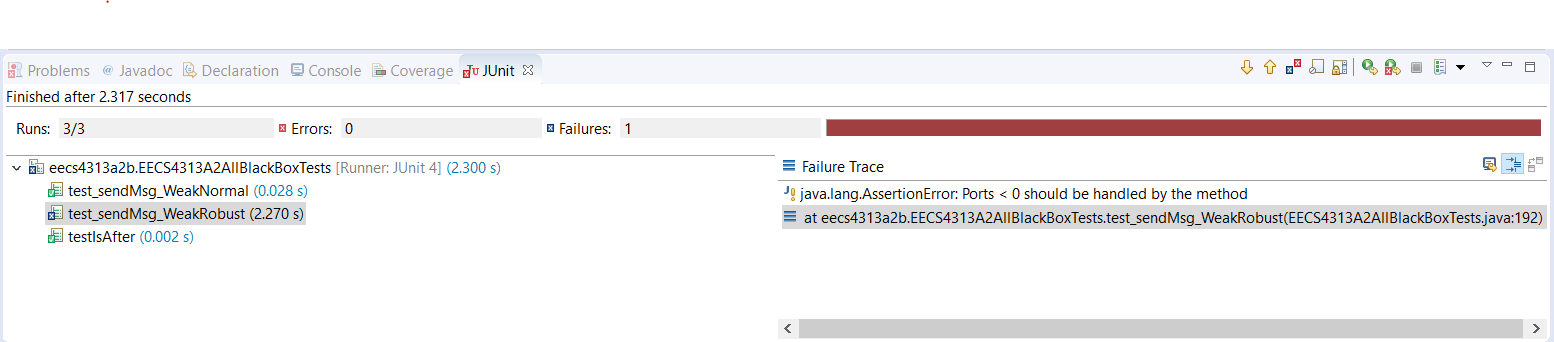
\includegraphics[width=.99\textwidth]{images/bbt/bvt-fail-1.png}
\end{center}
\caption{Test results using Weak Robust Boundary Value Testing}
\label{fig:bbt_bvt1}
\end{figure}

\begin{figure}[!htb]
\begin{center}
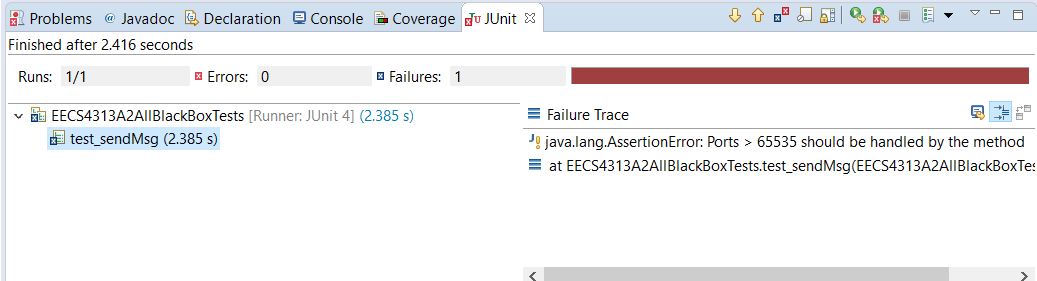
\includegraphics[width=.99\textwidth]{images/bbt/bvt-fail-2.png}
\end{center}
\caption{Test results using Weak Robust Boundary Value Testing}
\label{fig:bbt_bvt2}
\end{figure}

\begin{figure}[!htb]
\begin{center}
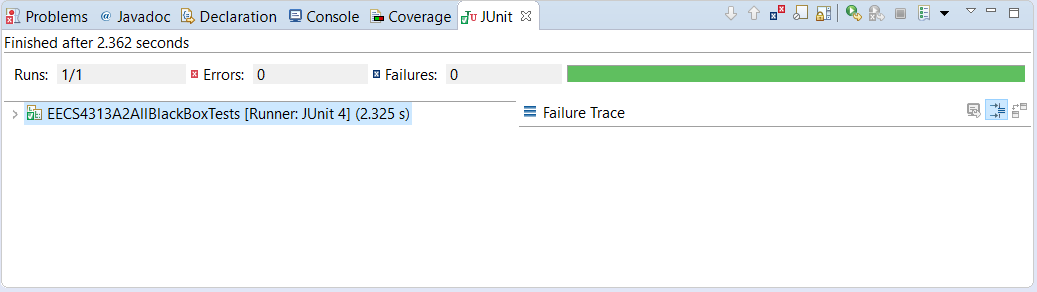
\includegraphics[width=.99\textwidth]{images/bbt/bvt-pass.png}
\end{center}
\caption{Test results using Weak Normal Boundary Value Testing}
\label{fig:bbt_bvt3}
\end{figure}

\newpage
\subsubsection{Testing Code}
\begin{lstlisting}
public class EECS4313A2AllBlackBoxTests implements SocketHandler {

	/**
	 * process a socket message
	 */
	@Override
	public synchronized String processMessage(String msg) {
		return msg;
	}
	@Test
	public void test_sendMsg_WeakNormal() {
		/** Method used: Boundary Value Testing **/
		String validHost = "localhost";

		int port_norm = 2929; // x_norm
		int port_min = 0; // x_min
		int port_min_plus = 1; // x_min+
		int port_max = 65535; // x_max
		int port_max_minus = 65534; // x_max-

		String response = "";
		// port_norm
		String msg = "Port 2929";
		SocketServer ss = new SocketServer(port_norm, this);
		try {
			response = SocketClient.sendMsg(validHost, port_norm, msg);
			assertEquals("Testing if a localhost on port_norm sends a message", response, msg);
		} catch (IOException e) {
			e.printStackTrace();
		}

		// port_min
		/*
		 * Throws connection problem. port 0 isn't available on my computer Connect
		 * Exception extends Socket Exception which extends IOException
		 */
		msg = "Port 0";
		try {
			ss = new SocketServer(port_min, this);
			response = SocketClient.sendMsg(validHost, port_min, msg);
			assertEquals("Testing if a localhost on port_min sends a message", response, msg);
		} catch (IOException e) {
			e.printStackTrace();
		}
		// port_min+
		msg = "Port 1";
		try {
			ss = new SocketServer(port_min_plus, this);
			response = SocketClient.sendMsg(validHost, port_min_plus, msg);
			assertEquals("Testing if a localhost on port port_min+ sends a message", response, msg);
		} catch (IOException e) {
			// TODO Auto-generated catch block
			e.printStackTrace();
		}

		// port_max
		msg = "Port 65535";
		try {
			ss = new SocketServer(port_max, this);
			response = SocketClient.sendMsg(validHost, port_max, msg);
			assertEquals("Testing if a localhost on port port_max sends a message", response, msg);
		} catch (IOException e) {
			// TODO Auto-generated catch block
			e.printStackTrace();
		}

		// port_max-
		msg = "Port 65534";
		try {
			ss = new SocketServer(port_max_minus, this);
			response = SocketClient.sendMsg(validHost, port_max_minus, msg);
			assertEquals("Testing if a localhost on port_max- sends a message", response, msg);

		} catch (IOException e) {
			// TODO Auto-generated catch block
			e.printStackTrace();
		}
	}

	@Test
	public void test_sendMsg_WeakRobust() {
		/** Method used: Boundary Value Testing **/
		String validHost = "localhost";

		int port_norm = 2929; // x_norm
		int port_min = 0; // x_min
		int port_min_plus = 1; // x_min+
		int port_max = 65535; // x_max
		int port_max_minus = 65534; // x_max-

		// robustness
		String invalidHost = "asdfasdf";
		int port_min_minus = -1; // x_min-
		int port_max_plus = 65536; // x_max_+

		String response = "";
		// port_norm
		String msg = "Port 2929";
		SocketServer ss = new SocketServer(port_norm, this);
		try {
			response = SocketClient.sendMsg(validHost, port_norm, msg);
			assertEquals("Testing if a localhost on port_norm sends a message", response, msg);
		} catch (IOException e) {
			e.printStackTrace();
		}
		/* Unknown host exception extends IOException */
		try {
			response = SocketClient.sendMsg(invalidHost, port_norm, msg);
			assertEquals("Testing if an invalid host on port_norm sends a message", response, msg);
		} catch (IOException e) {
			e.printStackTrace();
		}

		// port_min
		/*
		 * Throws connection problem. port 0 isn't available on my computer Connect
		 * Exception extends Socket Exception which extends IOException
		 */
		msg = "Port 0";
		try {
			ss = new SocketServer(port_min, this);
			response = SocketClient.sendMsg(validHost, port_min, msg);
			assertEquals("Testing if a localhost on port_min sends a message", response, msg);
		} catch (IOException e) {
			e.printStackTrace();
		}
		// port_min+
		msg = "Port 1";
		try {
			ss = new SocketServer(port_min_plus, this);
			response = SocketClient.sendMsg(validHost, port_min_plus, msg);
			assertEquals("Testing if a localhost on port port_min+ sends a message", response, msg);
		} catch (IOException e) {
			// TODO Auto-generated catch block
			e.printStackTrace();
		}

		// port_max
		msg = "Port 65535";
		try {
			ss = new SocketServer(port_max, this);
			response = SocketClient.sendMsg(validHost, port_max, msg);
			assertEquals("Testing if a localhost on port port_max sends a message", response, msg);
		} catch (IOException e) {
			// TODO Auto-generated catch block
			e.printStackTrace();
		}

		// port_max-
		msg = "Port 65534";
		try {
			ss = new SocketServer(port_max_minus, this);
			response = SocketClient.sendMsg(validHost, port_max_minus, msg);
			assertEquals("Testing if a localhost on port_max- sends a message", response, msg);

		} catch (IOException e) {
			// TODO Auto-generated catch block
			e.printStackTrace();
		}

		// port_min-
		/*
		 * Illegal argument Exception
		 */
		msg = "Port -1";
		try {
			ss = new SocketServer(port_min_minus, this);
			response = SocketClient.sendMsg(validHost, port_min_minus, msg);
			assertEquals("Testing if a localhost on port_min- sends a message", response, msg);
		} catch (IOException e) {
			e.printStackTrace();
		} catch (IllegalArgumentException iae) {
			fail("Ports < 0 should be handled by the method");
		}

		// port_max+
		/*
		 * Illegal argument Exception
		 */
		msg = "Port 65536";
		try {
			ss = new SocketServer(port_max_plus, this);
			response = SocketClient.sendMsg(validHost, port_max_plus, msg);
			assertEquals("Testing if a localhost on port_max+ sends a message", response, msg);
		} catch (IOException e) {
			e.printStackTrace();
		} catch (IllegalArgumentException iae) {
			fail("Ports > 65535 should be handled by the method");
		}
	}
\end{lstlisting}
\newpage
\subsubsection{Bug Report}
\begin{itemize}
\item \textbf{Bug Report Title}: Socket port values below 0 or above 65535 causes application to not be runnable after restart.
\item \textbf{Reported by}: Edward Vaisman
\item \textbf{Date reported}: March, 3rd, 2018
\item \textbf{Program (or component) name}: BORG Calendar version 1.8.3 - SocketServer Constructor, SocketClient sendMsg,  PrefName.SOCKETPORT
\item \textbf{Configuration(s)}:\\
\underline{System Info}
\begin{itemize}
\item{Operating System: Windows 10 Home 64-bit (10.0, Build 16299) (16299.rs3\_release.170928-1534)}
\item {Language: English (Regional Setting: English)}
\item {System Manufacturer: Dell Inc.}
\item {System Model: Inspiron 7559}
\item {Display Device: Intel(R) HD Graphics 530}
\item {Processor: Intel(R) Core(TM) i7-6700HQ CPU @ 2.60GHz (8 CPUs), ~2.6GHz }
\item {Memory: 8192MB RAM}
\item {BORG Calendar Version: 1.8.3}
\item {Java Version: 1.8.0\_161}
\end{itemize}
\underline{BORG Settings}
\begin{itemize}
\item{Socket Port: -2929}
\end{itemize}
\item \textbf{Report type}: Coding Error.
\item \textbf{Reproducibility}: 100\% (Tested on 4 seperate machines.)
\item \textbf{Severity}: High (Fatal)
\item \textbf{Problem summary}: After changing the socket port to -2929 and restarting the application causes BORG to be unusable even after a clean install.
\item \textbf{Problem description}:\\
Applying boundary value junit testing to the sendMsg method in SocketClient reveals that PrefName.SOCKETPORT is allowed to store socketports that aren't valid. As a result it causes an unhandled exception to throw in SocketClient and SocketServer when trying to use a port that isn't valid. The reproduction steps describe how to reach this bug within the application. \\
\underline{Steps to Reproduce in Application}
\begin{enumerate}

\item{Run the application}
\begin{figure}[!htb]
\begin{center}
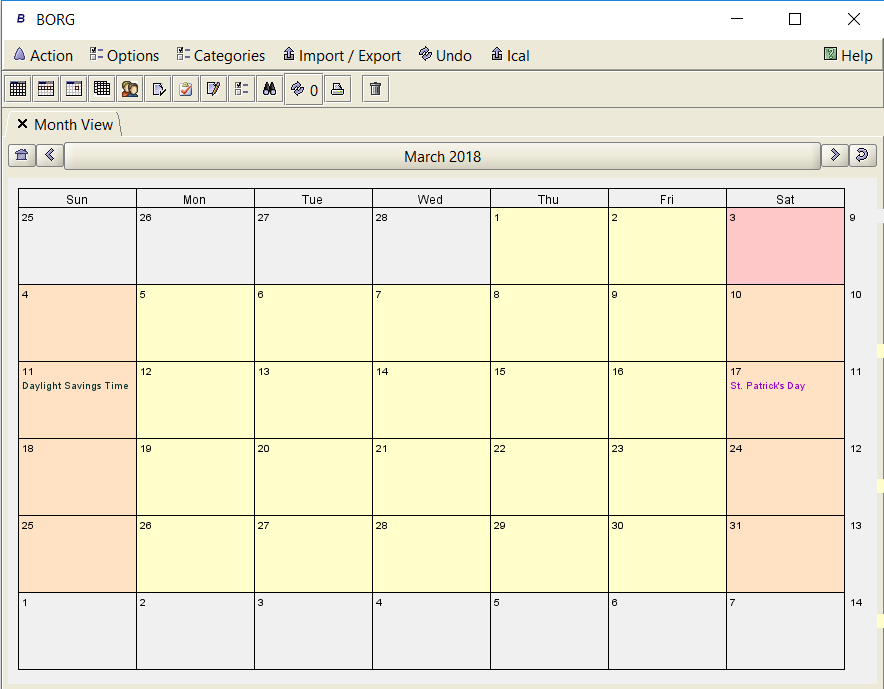
\includegraphics[width=.5\textwidth]{images/bbt/bvt-step1.png}
\end{center}
\caption{Run the application}
\label{fig:bbt_bvtstep1}
\end{figure}

\item{Select ``Options'' $\to$ ``Edit Preferences''.}
\begin{figure}[!htb]
\begin{center}
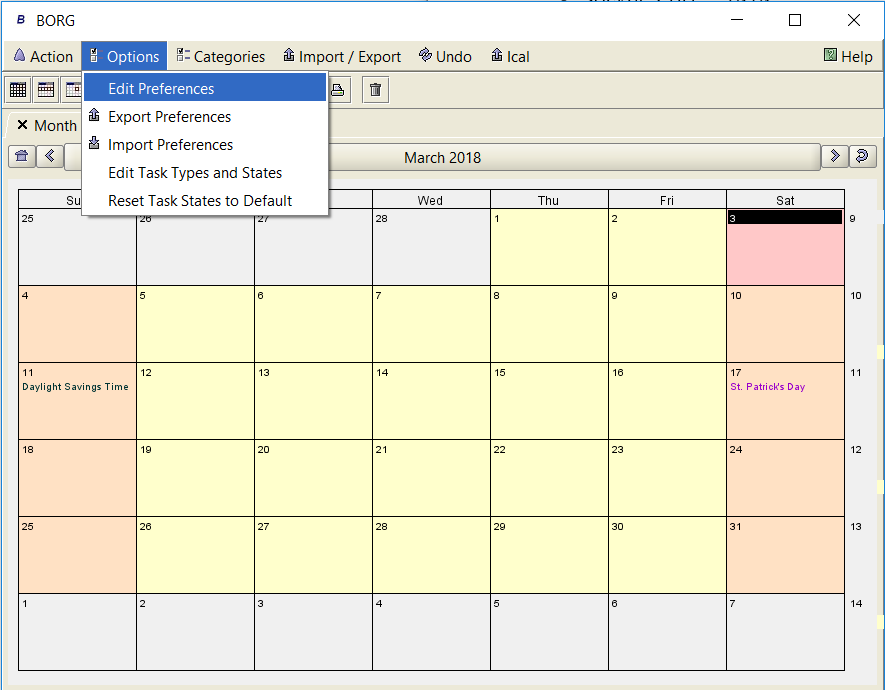
\includegraphics[width=.5\textwidth]{images/bbt/bvt-step2.png}
\end{center}
\caption{Opening the options window}
\label{fig:bbt_bvtstep2}
\end{figure}
\newpage
\item{The ``Options'' window appears. Select the ``Miscellaneous'' Tab.}
\begin{figure}[!htb]
\begin{center}
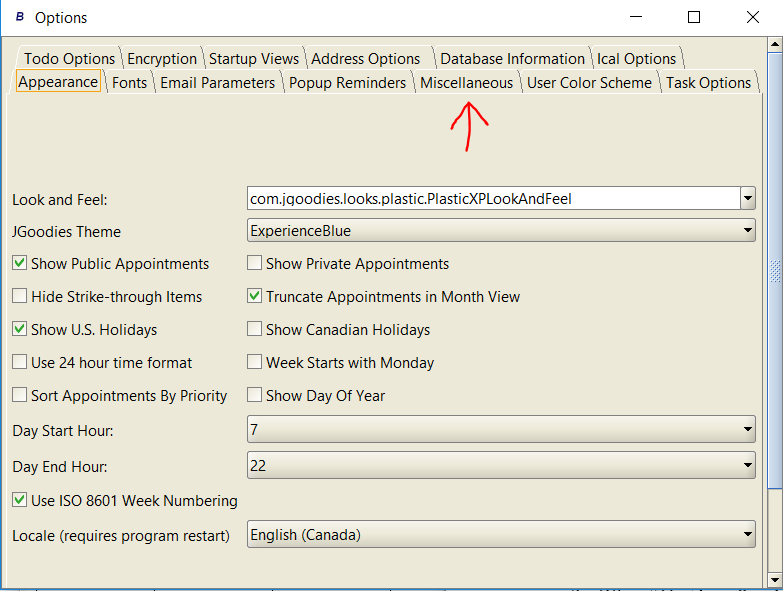
\includegraphics[width=.5\textwidth]{images/bbt/bvt-step3.png}
\end{center}
\caption{Selecting the Miscellaneous Tab}
\label{fig:bbt_bvtstep3}
\end{figure}

\item{Change Socket Port from 2929 to -2929 and press apply.}
\begin{figure}[!htb]
\begin{center}
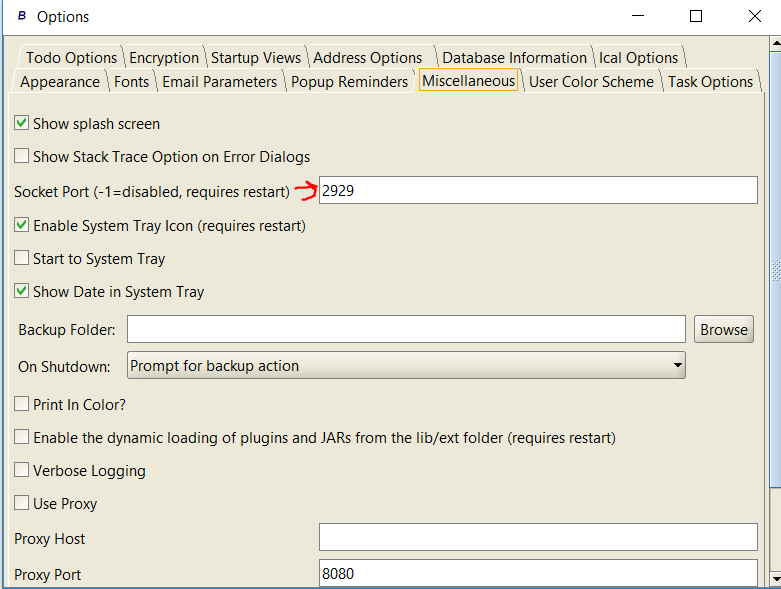
\includegraphics[width=.4\textwidth]{images/bbt/bvt-step4.png}
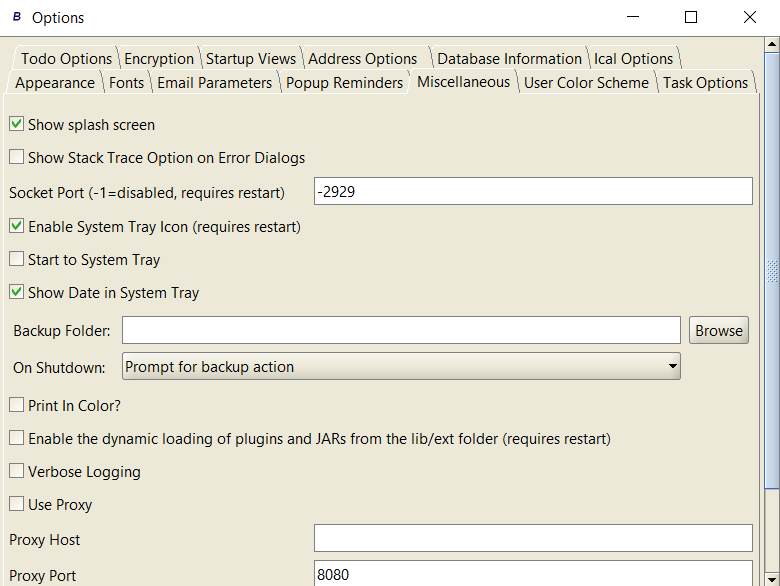
\includegraphics[width=.4\textwidth]{images/bbt/bvt-step4p2.png}
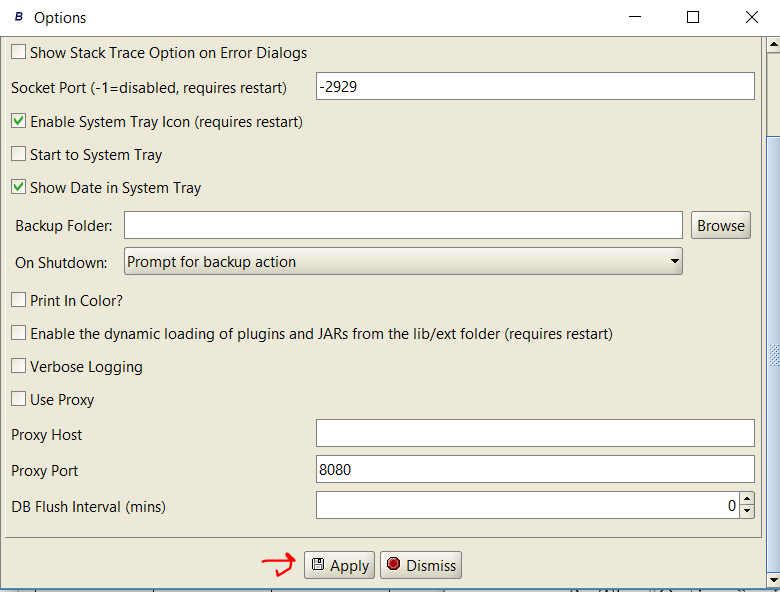
\includegraphics[width=.4\textwidth]{images/bbt/bvt-step5.png}
\end{center}
\caption{Changing the port (Part 1)}
\label{fig:bbt_bvtstep4}
\end{figure}

\item{Restart BORG.}
\end{enumerate}
\underline{Results}
\begin{itemize}
\item{Expected Results: Error message prompting the use of a valid socket port.}
\item{Real Results: Unable to run the application and thus not able to access calendar data.}
\begin{enumerate}
\item{Unable to run BORG after application restart}
\item{Unable to run BORG after clean uninstall and re-install}
\item{Unable to run BORG off a USB}
\item{Unable to run BORG after system restart}
\item{Unable to run BORG after java re-install}
\end{enumerate}
\end{itemize}
\underline{Additional Tests}\\
{Goals: To verify if the error only occurs with negative numbers/any port that is not 2929 or exactly with port -2929 or an error that occurs when attempting to change the port at all.}
\begin{enumerate}
\item{Attempt to reproduce with port 20. No errors.}
\item{Attempt to reproduce with port 1. No errors.}
\item{Attempt to reproduce with port -1. No errors.}
\item{Attempt to reproduce with port -20. Bug occured.}
\item{Attempt to reproduce by changing the port to -2929, applying the changes, and then setting it back to 2929 and applying changes. Bug occured.}
\item{Attempt to reproduce with port 65536. Bug occured.}
\end{enumerate}
\item \textbf{New or old bug}: New
\end{itemize}
\end{itemize}

\newpage
\subsection{Equivalence Class Testing}

\begin{itemize}
\item \textbf{Technique}: \emph{Equivalence Class Testing}
\item \textbf{Class}: \emph{net.sf.borg.common.DateUtil.java}
\item \textbf{Method}: \emph{minuteString(int mins)}
\item \textbf{Method Description}:
This method generate a human reable string for a particular numbe of minutes.It returns the string interms of hours or minutes or both hours and mintues.
\item \textbf{mins} - The argument is an integer
\item \textbf{Justification}: Equivalence class testing is suitable for this method since argument of this method is an integer which is an independent variable and the entire range of input can be partitioned while assuring disjointness and non-redundancy between each partition set. We have chosen these partition integer range based on when we use minute, minutes, hour, and hours.In order to partition the integer argument into hours and minutes,we divide the Minutes by 60 to get the range of hours and  the remainder ( minutes \% 60) to get the range of the minutes.The paritions for this method are:
 \begin{itemize}
\item \textbf{ Mins / 60 = 1 and Mins \% 60 = 0 :} To test 1 hour.
 \begin{itemize}
 \item Range of hours: [1]
 \item Range of minutes: [0]
\end{itemize}
\item \textbf{ Mins / 60 = 1 and Mins \% 60 = 1 :} To test the 1 hour with 1 minute.
 \begin{itemize}
 \item Range of hours: (1,$+\infty$)
 \item Range of minutes: [1]
\end{itemize}
\item \textbf{ Mins / 60 = 1 and Mins \% 60  $>$  1 :} To test 1 hour with minutes more than 1 minute. 
 \begin{itemize}
 \item  Range of hours: [1]
\item  Range of Minutes : (1, 59]
\newpage
\end{itemize}
\item \textbf{ Mins / 60 $>$ 1 and Mins \% 60 = 0 :} To test the hours more than 1 hour.
 \begin{itemize}
 \item Range of hours: (1,$+\infty$)
 \item Range of minutes: [0]
\end{itemize}
\item \textbf{ Mins / 60 $>$ 1 and Mins \% 60 = 1 :} To test hours more than 1 hour with 1 minute. 
 \begin{itemize}
 \item Range of hours: (1,$+\infty$)
\item Range of Minutes :[1]
\end{itemize}
\item \textbf{ Mins / 60 $>$ 1 and Mins \% 60 $>$ 1 :} To test the hours more than 1 hour with minutes more than 1 minute. 
 \begin{itemize}
 \item Range of hours:  (1,$+\infty$) 
\item Range of Minutes : (1, 59]
\end{itemize}
\item \textbf{ Mins / 60 = 0 and Mins \% 60 = 0 :} To test 0 minutes.
 \begin{itemize}
 \item Range of hours: [0]
 \item Range of minutes: [0]
\end{itemize}
\item \textbf{ Mins / 60 = 0 and Mins \% 60 = 1 :} To test 1 minute.
 \begin{itemize}
 \item Range of hours: [0]
 \item Range of minutes: [1]
\end{itemize}
\item \textbf{ Mins / 60 = 0 and Mins \% 60 $>$ 1 :} To test minutes more than 1 minute and less than 60 minutes or 1 hour.
 \begin{itemize}
 \item Range of hours: [0]
 \item Range of minutes: (1,59]
\end{itemize}
\end{itemize}
The method did not specifity how negative minutes should be treated, so we omit  the negative integers as an argument for this method.For example, -75 can be converted as -1 hour and 15 minutes or 45 minutes or any other way. Therefore, this case is tested in the whitebox testing after analyzing structure of the method.
\item \textbf{Evaluation :}  The tests are shown below suitable for strong normal equivalence class testing technique since it covers the all the range of outputs for valid inputs and invalid inputs (negative integers) are not tested due to lack of specfication information regarding these values. 
\newpage
 \begin{itemize}
\item \textbf{Class 1:} Mins / 60 = 1 and Mins \% 60 = 0 
\item \textbf{Class 2:}  Mins / 60 = 1 and Mins \% 60 = 1
\item \textbf{Class 3:} Mins / 60 = 1 and Mins \% 60  $>$  1
\item \textbf{Class 4:} Mins / 60 $>$ 1 and Mins \% 60 = 0
\item \textbf{Class 5:} Mins / 60 $>$ 1 and Mins \% 60 = 1
\item \textbf{Class 6:} Mins / 60 $>$ 1 and Mins \% 60 $>$ 1
\item \textbf{Class 7:} Mins / 60 = 0 and Mins \% 60 = 0
\item \textbf{Class 8:} Mins / 60 = 0 and Mins \% 60 = 1
\item \textbf{Class 9:} Mins / 60 = 0 and Mins \% 60 $>$ 1
\end{itemize}
\begin{figure}[!htb]
\begin{center}
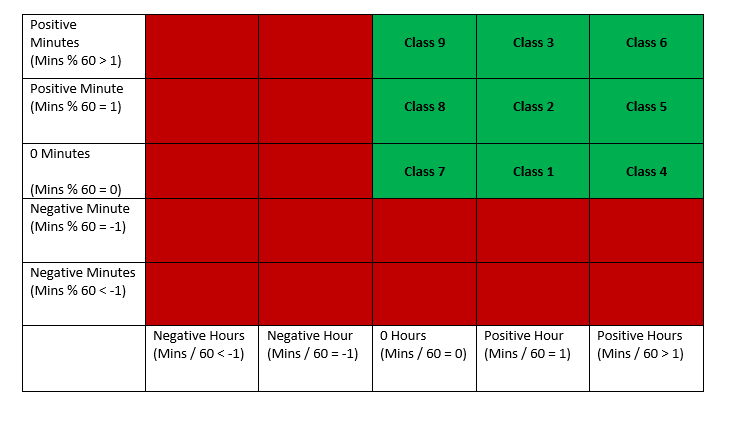
\includegraphics[width=.99\textwidth]{images/bbt/bbtmatrix.png}
\end{center}
\caption{Proving the test cases produce Strong Normal ECT}
\label{fig:bbt_matrix}
\end{figure}
In the Figure 1, The boxes colored in green represent all the valid output results and red boxes represent the invalid results which cannot be tested since the method did not specify how the negative integers should be treated. The Class 1,Class 2....Class 9 represents the partitions that we derived from how to convert the integers into readable string.
\newpage
\begin{figure}[!htb]
\begin{center}
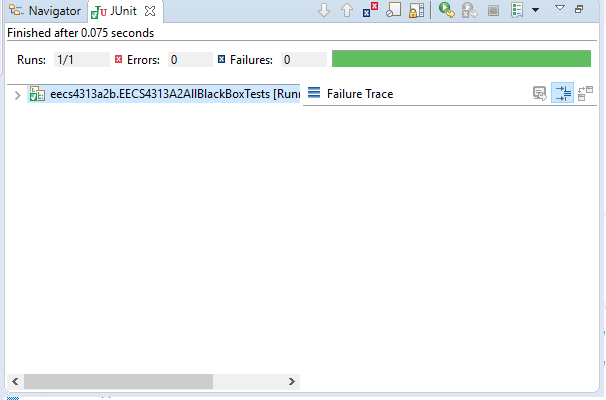
\includegraphics[width=.99\textwidth]{images/bbt/bbt_ect.png}
\end{center}
\caption{Test results using Strong Normal ECT}
\label{fig:bbt_ect}
\end{figure}

\newpage
\subsubsection{Testing Code}
\begin{lstlisting}
package eecs4313a2b;

import static org.junit.Assert.*;

import org.junit.Test;

import net.sf.borg.common.DateUtil;

public class EECS4313A2AllBlackBoxTests {

	@Test
	public void testMinuteString() {

		// Hour
		// Class 1: Mins/60 = 1 and Mins\%60 = 0 - Testing 1 hour [Range: [1]]
		assertEquals("1 Hour", DateUtil.minuteString(60));
		// Class 2: Mins/60 = 1 and Mins\%60 = 1 -Testing 1 hour with 1 minute [Range:[1] hour and [1] minute]
		assertEquals("1 Hour 1 Minute", DateUtil.minuteString(61));
		// Class 3: Mins/60 = 1 and Mins\%60 > 1 -Testing 1 hour with some minutes [Range:[1] hour and (1,59] minutes]
		assertEquals("1 Hour 15 Minutes", DateUtil.minuteString(75));
		// -------------------------------------------------------
		// Hours
		// Class 4: Mins/60 > 1 and Mins\%60 = 0 -Testing hours more than one [Range:(1, infinity) hours]
		assertEquals("3 Hours", DateUtil.minuteString(180));
		// Class 5: Mins/60 > 1 and Mins\%60 = 1 -Testing hours more than 1 hour with some minutes [Range:(1,infinity) hours and [1] minute]
		assertEquals("2 Hours 1 Minute", DateUtil.minuteString(121));
		// Class 6: Mins/60 > 1 and Mins\%60 > 1 -Testing hours more than 1 hour with some minutes [Range:(1,infinity) hours and (1,59] minutes]
		assertEquals("2 Hours 25 Minutes", DateUtil.minuteString(145));
		// --------------------------------------------------------
		// Minutes
		// Class 7: Mins/60 = 0 and Mins\%60 = 0 -Testing 0 minutes [Range:[0] minute]
		assertEquals("0 Minutes", DateUtil.minuteString(0));
		// Class 8: Mins/60 = 0 and Mins\%60 = 1 -Testing 1 minute [Range:[1] minute]
		assertEquals("1 Minute", DateUtil.minuteString(1));
		// Class 9: Mins/60 = 0 and Mins\%60 > 1 - Testing minutes that are less than 1 hour [Range: (1,59] minutes]
		assertEquals("50 Minutes", DateUtil.minuteString(50));
	}
}



\end{lstlisting}

\end{itemize}

\newpage
\subsection{Decision Table Testing}

\begin{itemize}
\item \textbf{Technique}: \emph{Decision Table Testing}
\item \textbf{Class}: \emph{net.sf.borg.common.DateUtil.java}
\item \textbf{Method}: \emph{isAfter(Date d1, Date d2)}
\item \textbf{Method description}: The method checks if a given date \emph{d1} falls on a later calendar day than date \emph{d2}. It returns \textbf{true} if \emph{d1} does fall on a later calendar day than \emph{d2} and \textbf{false} otherwise.
\begin{itemize}
\item \textbf{d1} - The first argument is of type Java Date Object.
\item \textbf{d2} - The second argument is of type Java Date Object.
\end{itemize}
\item \textbf{Justification}: Decision table testing technique is an appropriate testing technique for this method because there are decision making to be done among the input variables. It consists of logical relationships among the input variables, i.e date \emph{d1} appearing before, after or at the same time as date \emph{d2}, which directly affects the output.
\end{itemize}

\begin{table}[h]
\centering
\begin{tabular}{|c | c | c | c | c | c | c | c |}
	\cline{1-8}
	& \textbf{Rule 1-2} & \textbf{Rule 3} & \textbf{Rule 4} & \textbf{Rule 5} & \textbf{Rule 6} & \textbf{Rule 7} & \textbf{Rule 8}\\ \hline
	C1: d1 $<$ d2 & T & T & T & F & F & F & F \\ \hline
	C2: d1 $=$ d2 & T & F & F & T & T & F & F \\ \hline
	C3: d1 $>$ d2 & - & T & F & T & F & T & F \\ \Xhline{2pt}
	A1: Date is after & & & & & & X & \\ \hline
	A2: Date is not after & & & X & & X & & \\ \hline
	A3: Impossible & X & X & & X & & & X \\ \hline
\end{tabular}
\caption {Decision Table for the isAfter method}
\label{tbl:trace_matrix}
\end{table}

\noindent \textbf{Rationale}: The decision table above outlines 8 rules. The rules are derived from three equivalence classes: d1 is less than d2, d1 is equal to d2 and d1 is greater than d2. Each equivalence class can have 2 different values (i.e T or F), giving us $2^3 = 8$ rules. Out of the 8 rules, 5 of the rules points to \emph{Impossible} cases, hence cannot be converted to test cases. The other 3 rules are converted into test cases. Below is the code snippet and the test run screenshot for the test cases derived using the decision table technique.

\newpage
\subsubsection{Testing Code}
\begin{code}
	@Test
	public void testIsAfter() {
		/** Method used: Decision Table Testing **/
		
		Date d1 = new Date(117, 11, 3);
		Date d2 = new Date(117, 11, 3);
		boolean result;
		
		// date d1 is equal to d2
		result = DateUtil.isAfter(d1, d2);
		assertFalse("Date d1 is equal to d2", result);
		
		// date d1 is before d2
		d1.setDate(2);
		result = DateUtil.isAfter(d1, d2);
		assertFalse("Date d1 is before d2", result);
		
		// date d1 is after d2
		d1.setDate(4);
		result = DateUtil.isAfter(d1, d2);
		assertTrue("Date d1 is after d2", result);
	}
\end{code}

\begin{figure}[!htb]
\begin{center}
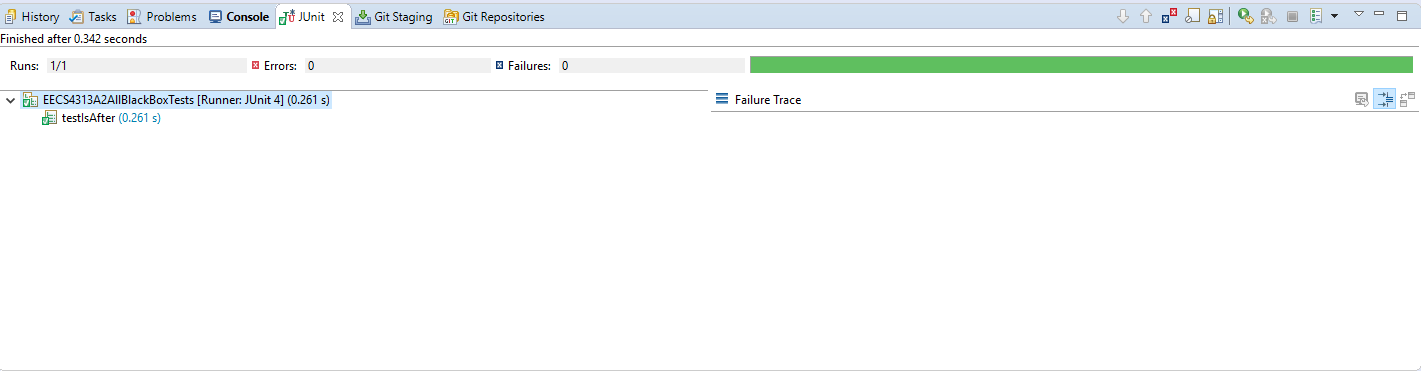
\includegraphics[width=.99\textwidth]{images/bbt/dtt.png}
\end{center}
\caption{Test results using Decision Table Testing Technique}
\label{fig:bbt_dtt}
\end{figure}

\newpage
\section{White Box Testing}

\begin{itemize}
\item The statement coverage measurements for your Assignment 2 test suite.
\item A description of the test cases that you added in this assignment to improve statement
coverage. The marker will not read your code in order to see what you tested. You have to
describe it.
\item The statement coverage measurements for your final submission. Include the screenshots of
the test running results and the screenshots of the coverage measurement. If your coverage is
not 100%, include a discussion on why that is.
\item The Control Flow Graph you created. Indicate the segments clearly (you will probably need
to include the code for this).
\item The path coverage discussion described in section 2 above.
\item Attaching bug reports if bugs are discovered using your testing methods. You should use the
same bug report format as in Assignment 1. Do not file these bug reports to the project’s bug
report system.
\item An appendix with the specification of the methods you are testing (if there are new ones). 
\end{itemize}

\end{document}
